\section{Zielsetzung}
In diesem Versuch wird die Funktionsweise eines Helium-Neon Lasers untersucht. Dafür werden nach einer Justage des Lasers 
verschiedene Eigenschaften des Laserlichts, wie die Wellenlänge oder TEM-Moden vermessen.

\section{Theorie}
\label{sec:Theorie}

Der Begriff \texttt{LASER} ist ein Akronym für \textit{Light amplification by stimulated emission of radiation}. Laser zeichnen als
leistungsstarke Quelle von monochromatischem Licht aus und finden daher häufig in verschiedenen Experimenten Anwendung. Für einen Laserbetrieb werden grundsätzlich
drei Komponenten benötigt: eine Besetzungsinversion, ein aktives Medium, in dem stimulierte Emission stattfinden kann, und einen Resonator. Die theoretischen
Grundlagen der Komponenten und der Aufbau eines Helium-Neon Lasers (HeNe-Laser) werden hier erörtert.

\subsection{Zustandssysteme und Besetzungsinversion}
Um die Funktionsweise eines Lasers zu vestehen, ist ein Blick auf die quantenmechanische Beschreibung von Zustandssystemen notwendig.
In der Quantenmechanik wird werden Zustände von Teilchen einer bestimmten Energie zugeordnet, sodass unterschiedliche Zustände verschiedene
Energien besitzen. Es ergibt sich ein Zustandssytem, in dem die Teilchen durch Absorbtion und Emission von Photonen in Zustände höherer Energie wechseln können,
wenn die Energie der anregenden (Quasi-)Teilchen
\begin{equation}
    E = h\nu
\end{equation}
genau der Energiedifferenz zweier Zustände entspricht.

Befinden sich mehr Teilchen in einem höheren Energiezustand als dem Grundzustand, wird von \textit{Besetzungsinversion} gesprochen. Diese kann
nur für ein Zustandssystem mit mehr als 2 Zuständen erreicht werden, da hier die Übergangswahrscheinlichkeiten $E_1 \rightarrow E_2 ≤ E_2 \rightarrow E_1$
maximal eine Gleichverteilung zulassen.

In einem Zustandssystem mit mehr als zwei Energieniveaus ist es hingegen möglich, durch hinreichende äußere Anregung eine Besetzungsinversion zu erreichen. 
Die äußere Anregung wird auch als \textit{pumpen} bezeichnet.

\subsection{Zustandssystem von Helium und Neon}
Für das in \autoref{fig:Zustandssystem_HeNe} gezeigte Zustandssysten von Helium und Neon kann eine Besetzungsinversion erreicht werden.
Durch Stöße mit Elektronen wird Helium aus seinem Grundzustand in 
die Zustände $2^1\symup{s}$ und $2^3\symup{s}$ gehoben. Die angeregten Heliumatome heben durch Stöße die Neonatome in die Zustände $5\symup{s}$ und $4\symup{s}$.
Dies erzeugt die gewünschte Besetzungsinversion in den Zuständen der Neonatome.

\begin{figure}
    \centering
    \includegraphics[width=0.9\textwidth]{content/pics/Zustandssystem_HeNe.pdf}
    \caption{Ausschnitt des Zustandssystem von Helium und Neon. Durch Elektronenströße angeregte Heliumatome können durch Stöße mit Neonatomen ihre Energie
    übertragen und so eine Besetzungsinversion erzeugen \cite{Zustandssystem_HeNe}.}
    \label{fig:Zustandssystem_HeNe}
\end{figure}

\subsection{Spontane und stimulierte Emission}
Befinden sich Teilchen in einem angeregten Zustand können diese in einen Zustand niederer Energie übergehen, indem ein Photon mit der Wellenlänge zu der korrenspondierenden
Energielücke emittiert wird. Dies geschieht nach einer systemspezifischen Zeit durch spontane Emission, wobei das endsandte Photon keine ausgezeichnete Phasenlage,
Polarisation oder Richtung aufweist.
Trifft ein Photon mit derselben Energie wie die Energielücke zwischen den Zuständen auf ein Atom im angeregten Zustand, kann es zu stimulierter Emission kommen.
Dabei regt das eintreffende Photon die Emission eines weiteren Photons selber Energie, Richtung, Polarisation und Phasenlage an. Die beiden Photonen sind kohärent 
zueinander. In \autoref{fig:Stimulierte_Emission} ist dies graphisch dargestellt.

\begin{figure}
    \centering
    \includegraphics[height=4cm]{content/pics/Stimulierte_Emission.png}
    \caption{Beispiele von spontaner und stimulierter Emission eines Photons beim Übergang eines Teilchens in einen Zustand niedrigerer Energie \cite{Stimulated_Emission}.}
    \label{fig:Stimulierte_Emission}
\end{figure}

\subsection{Resonator}
Für die erwünschte stimulierte Emission werden Photonen mit der richtigen Energie benötigt, welche die Emission weiterer Photonen induzieren. Dafür wird ein 
Resonator benötigt, der aus zwei Spiegeln besteht. Das austretende Licht wird zurück ins das aktive Medium reflektiert, sodass dort erneut stimulierte Emission
ausgelöst werden kann. Über einen der beiden Spiegel wird ein kleiner Teil des Lichts in der Größenordnung von \qty{1}{\percent} ausgekoppelt. Dies ist das Laserlicht,
welches für verschiedene Experimente verwendet werden kann. In \autoref{fig:Laserschema} ist der grundsätzlich Aufbau eines Lasers dargestellt.

\begin{figure}
    \centering
    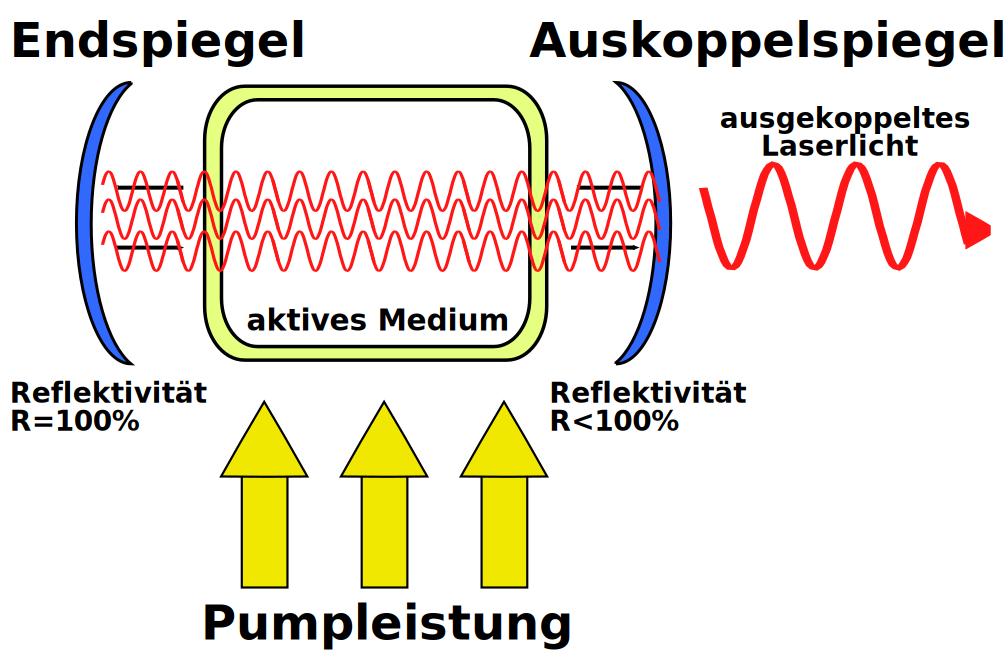
\includegraphics[height=6cm]{content/pics/Laserschema.pdf}
    \caption{Skizze des Funktionsprinzip eines Lasers. Zwei Spiegel reflektieren den Großteil des Lichts zurück in das aktive Medium und funktionieren so
    als Resonator \cite{Laserschema}.}
    \label{fig:Laserschema}
\end{figure}

Als Spiegel können sowohl konfokale, als auch planare Formen verwendet werden. Auch der Abstand der Spiegel ist variabel, wobei die Brennpunkte der Spiegel zu beachten sind.
Wird nicht genügend Licht in das aktive Medium zurückreflektiert, kommt es nicht in ausreichendem Maße zu stimulierter Emission, sodass kein Laserbetrieb stattfindet.
Zur Beschreibung der Stabilität der Resonatoranordnung wird Lasers werden so genannte $g$-Faktoren

\begin{equation}
    g_{\symup{i}} = \frac{L}{r_{\symup{i}}}
    \label{eq:g_i}
\end{equation}
eingeführt. Hierbei bezeichnet $L$ die Länge des Resonators, also den Abstand der beiden Spiegel, und $r$ den Krümmungsradius dieser. Für einen planaren Spiegel wird ein unendlich großer
Krümmungsradius angenommen.

Aus optischen Überlegungen ergibt sich eine Stabilitätsbedingung für den Resonator. Damit ausreichend stimulierte Emission passiert, muss

\begin{equation}
    0 ≤ g_1g_2 ≤ 1
    \label{eq:g1g2}
\end{equation}

gelten. Die Faktoren $g_1$ und $g_2$ werden mit \eqref{eq:g_i} berechnet.

\subsection{TEM-Moden}
Das erzeugte Laserlicht hat eine sehr viel kleinere Wellenlänge als die Länge des Resonators, sodass mehrere Frequenzen im Resonator eine stehende Welle bilden können. Diese unterschiedlichen
Frequenzen werden als longitudinale Moden bezeichnet. 

Aufgrund von kleinen Unebenheiten oder Verdrehungen der Spiegel können auch transversalen Moden beobachtet werden.

\subsection{Brechung am Gitter}

\begin{equation}
    n \lambda = g \sin(\varphi_n)
    \label{eq:Interferenzbedingung}
\end{equation}

\begin{equation}
    \lambda = \frac{g\sin\left(\tan\left(\frac{s_{\symup{n}}}{2d}\right)\right)}{n}
    \label{eq:lambda}
\end{equation}